\subsection{User Management - FR1}

%Profiel Aanmaken
\subsubsection{Profiel aanmaken}
	\begin{table}[H]
	\caption{FR1.1 - Profiel aanmaken}
    		\begin{tabular}{l | p{10cm}}
        \textbf{ID:} & FR1.1 \\ \hline
        \textbf{TITEL:} & Profiel aanmaken \\ \hline
        \textbf{PRIORITEIT:} &  Hoog \\ \hline
        \textbf{PREREQUISITIES:} & Geen\\ \hline
        \textbf{TOEGANG:} &  Gast \\ \hline
        \textbf{BESCHRIJVING:} & Gebruiker zal zijn persoonlijke informatie moeten ingeven:
                                    \begin{itemize}\itemsep1pt \parskip0pt \parsep0pt
                                        \item Naam
                                        \item Voornaam
                                        \item Gebruikersnaam
                                        \item Wachtwoord
                                        \item Geboortedatum
                                        \item E-mail
                                        \item Rolnummer (optioneel)
                                        \item Richting (= vaste lijst) (optioneel)
                                        \item Gewenste taal
                                    \end{itemize}\\
    \end{tabular} 
	\label{tab:FR1.1 -Profiel aanmaken}
\end{table}

\textbf{Stappenplan:}
\begin{enumerate}
\item De niet-aangemelde gebruiker (voortaan gebruiker geheten) ziet het beginvenster (zie figuur \ref{fig:CalZone Home}) van de applicatie in zijn webbrowser.
\item De gebruiker klikt op de aanwezige knop om een profiel aan te maken.
\item De gebruiker krijgt een formulier te zien (zie figuur \ref{fig:CalZone Register}) met invulbare velden voor zijn naam, voornaam, gebruikersnaam, wachtwoord, geboortedatum, email. 
\item De gebruiker vult al de gegevens en selecteert de juiste optie in elke lijst.
\item Nadat de gebruiker deze gegevens volledig heeft ingevuld, klikt hij op de knop om de aanmaak van het profiel te beëindigen.
\item De gebruiker krijgt een melding op het scherm te zien dat het aanmaken van het profiel voltooid is.
\item Het systeem stuurt een email naar het opgegeven emailadres ter bevestiging (zie figuur \ref{fig:CalZone Activation}).
\end{enumerate}

%TODO
\textbf{Uitzonderingen:}
\begin{itemize}
\item Gegevens onvolledig ingevuld
\end{itemize}

\begin{center}
\begin{figure}[H]
\caption{CalZone Home}
\centerline{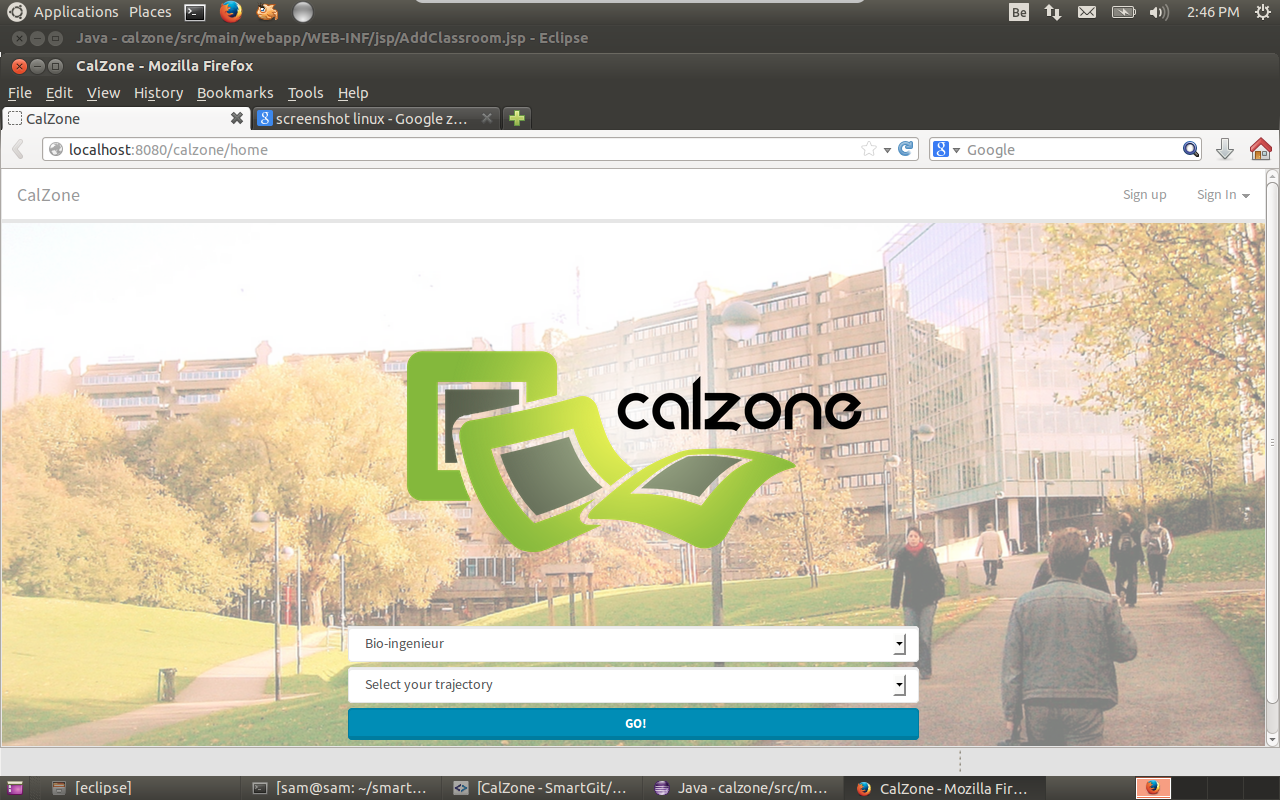
\includegraphics[scale=0.4]{img/CalzoneHome}}
\label{fig:CalZone Home}
\end{figure}

\begin{figure}[H]
\caption{CalZone Register}
\centerline{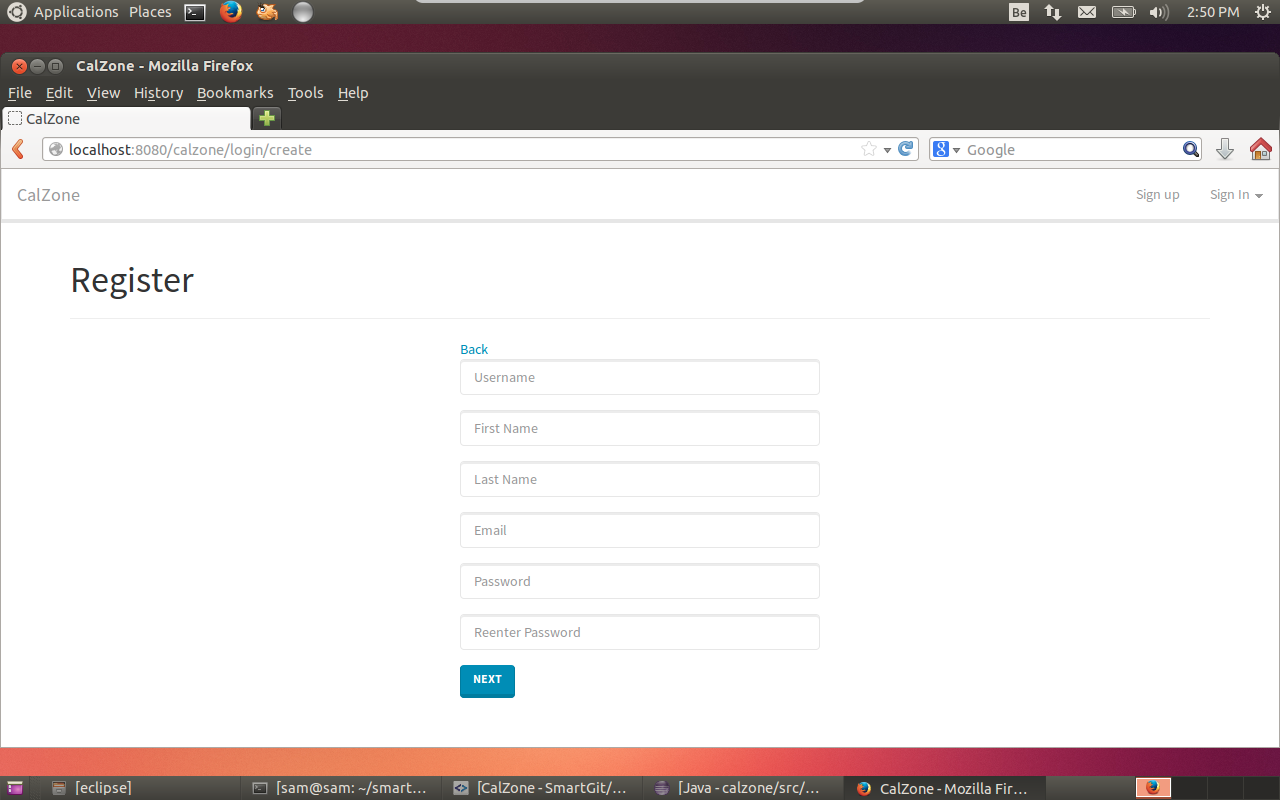
\includegraphics[scale=0.4]{img/CalzoneRegister}}
\label{fig:CalZone Register}
\end{figure}

\begin{figure}[H]
\caption{CalZone Activation}
\centerline{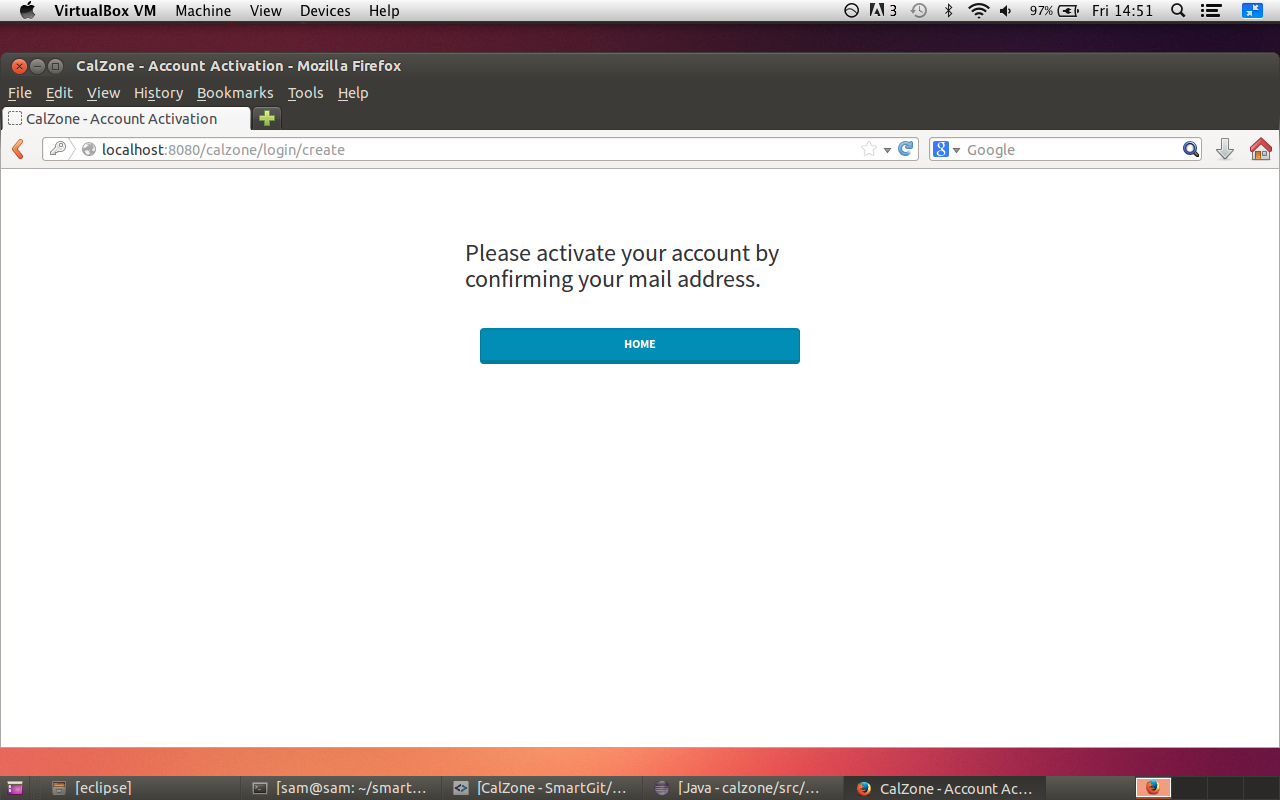
\includegraphics[scale=0.4]{img/CalzoneActivation}}
\label{fig:CalZone Activation}
\end{figure}
\end{center}

%Aanmelden
\subsubsection{Aanmelden}
\noindent\begin{table}[H]
            \begin{tabular}{l | p{10cm}}
                \textbf{ID:} & FR1.2 \\ \hline
                \textbf{TITEL:} & Aanmelden \\ \hline
                \textbf{PRIORITEIT:} &  Hoog \\ \hline
                \textbf{PREREQUISITIES:} & Gebruiker moet profiel bezitten\\ \hline
                \textbf{TOEGANG:} &  Gast \\ \hline
                \textbf{BESCHRIJVING:} & Gebruiker vult zijn username en wachtwoord in en klikt op “aanmelden”\\
            \end{tabular}
            \caption{FR1.2 - Aanmelden}
            \label{tab:FR1.2 - Aanmelden}
        \end{table}
        
\textbf{Stappenplan:}
\begin{enumerate}
\item De niet-aangemelde gebruiker (voortaan gebruiker geheten) ziet het beginvenster (zie figuur \ref{fig:CalZone Home}) van de applicatie in zijn webbrowser . Hier ziet de gebruiker een formulier met 2 velden om zijn gebruikersnaam en wachtwoord in te typen met daaronder een knop om in te loggen
\item De gebruiker vult zijn gebruikersnaam en wachtwoord in.
\item De gebruiker klikt op de knop om in te loggen.
\item De gebruiker is ingelogd en ziet nu zijn persoonlijk hoofdpagina (zie figuur \ref{fig:CalZone Profile}).
\end{enumerate}

%TODO
\textbf{Uitzonderingen:}
\begin{itemize}
\item Ingevoerde gebruikersnaam is niet gevonden.
\item Ingevoerd wachtwoord is verkeerd.
\end{itemize}

\begin{center}
\begin{figure}[H]
\caption{CalZone Profile}
\centerline{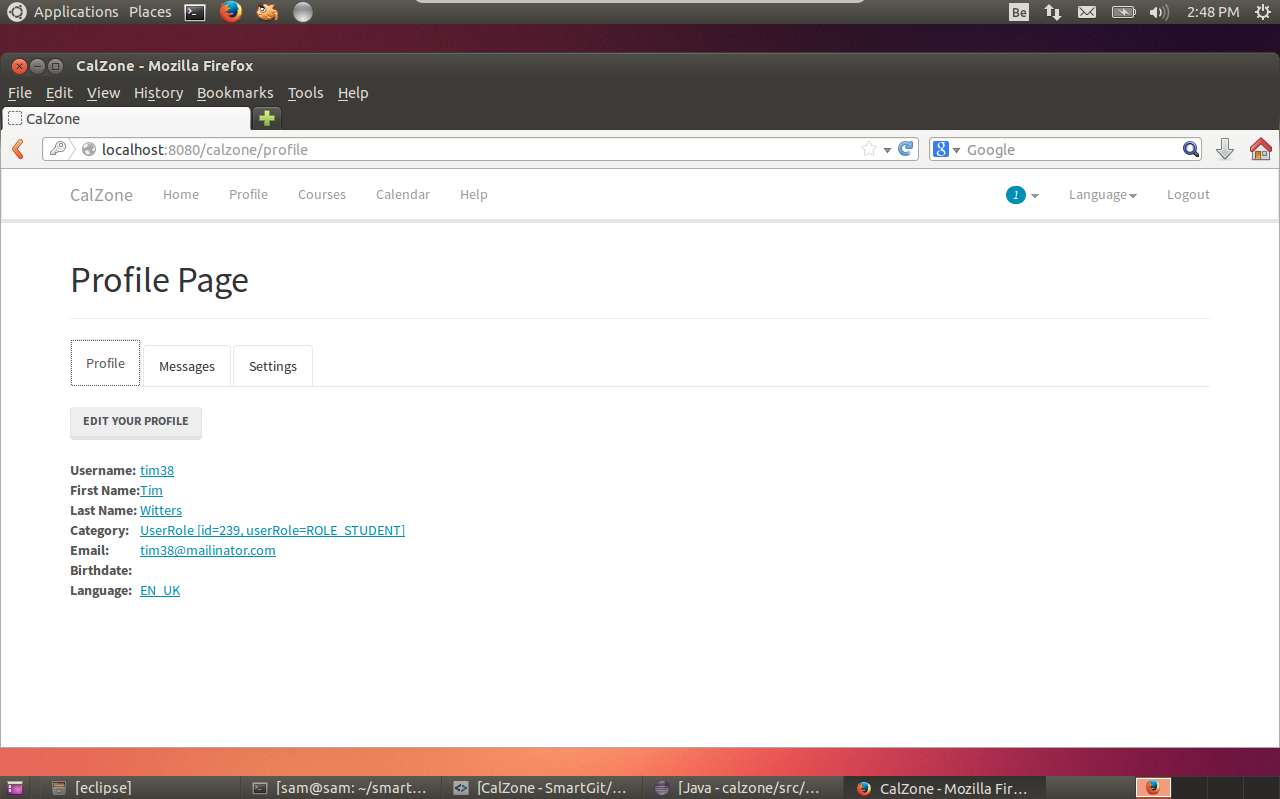
\includegraphics[scale=0.4]{img/Calzoneprofile}}
\label{fig:CalZone Profile}
\end{figure}
\end{center}

%Wachtwoord vergeten
\subsubsection{Wachtwoord vergeten}
\noindent\begin{table}[H]
            \begin{tabular}{l | p{10cm}}
                \textbf{ID:} & FR1.3 \\ \hline
                \textbf{TITEL:} & Wachtwoord vergeten \\ \hline
                \textbf{PRIORITEIT:} &  Medium \\ \hline
                \textbf{PREREQUISITIES:} & Gebruiker moet profiel bezitten\\ \hline
                \textbf{TOEGANG:} &  Niet-aangemelde gebruiker \\ \hline
                \textbf{BESCHRIJVING:} & Mocht een gebruiker zijn wachtwoord vergeten, dan moet deze zijn e-mail adres invoeren. 
                                        Hierna zal een e-mail met een reset link verstuurd worden naar het ingevoerde e-mail adress. 
                                        Als e-mail adress niet bestaat dient er een error bericht gegeven te worden aan de gebruiker\\
            \end{tabular}\\
            \caption{FR1.3 - Wachtwoord vergeten}
            \label{tab:FR1.3 - Wachtwoord vergeten}
        \end{table}

\textbf{Stappenplan:}
\begin{enumerate}
\item De niet-aangemelde gebruiker (voortaan gebruiker geheten) ziet het beginvenster (zie figuur \ref{fig:CalZone Home}) van de applicatie in zijn webbrowser. Hier ziet de gebruiker een knop met de tekst "Wachtwoord vergeten?".
\item De gebruiker klikt op deze knop. Er verschijnt een nieuw venster op het scherm (zie figuur \ref{fig:CalZone Lost Password 1}), met de vraag om het mailadres van zijn profiel in te vullen in het formulier op hetzelfde scherm.
\item Het systeem verstuurt een email naar het opgegeven mailadres met als inhoud een "resetlink", een speciale URL om het wachtwoord tijdelijk te kunnen wijzigen.
\item De gebruiker opent de \"resetlink\" in de e-mail en krijgt een venster te zien in zijn webbrowser (zie figuur \ref{fig:CalZone Lost Password 2}) met een formulier om het nieuwe wachtwoord in te voeren en deze te bevestigen.
\item De gebruiker vult het nieuwe wachtwoord in en bevestigd deze door ze op exact dezelfde schrijfwijze in te voeren in het tweede veld van het formulier.
\item De gebruiker klikt op de knop met de naam "Wachtwoord wijzigen" om de wijziging door te voeren.
\item De gebruiker krijgt een melding op het scherm dat het wachtwoord is gewijzigd en wordt terug naar het beginscherm van de applicatie geleid.
\end{enumerate}

%TODO
\textbf{Uitzonderingen:}
\begin{itemize}
\item Mailadres bestaat niet.
\item Wachtwoord voldoet niet aan de minimale vereisten.
\item Wachtwoord is foutief bevestigd.
\end{itemize}

\begin{center}
\begin{figure}[H]
\caption{CalZone Lost Password 2}
\centerline{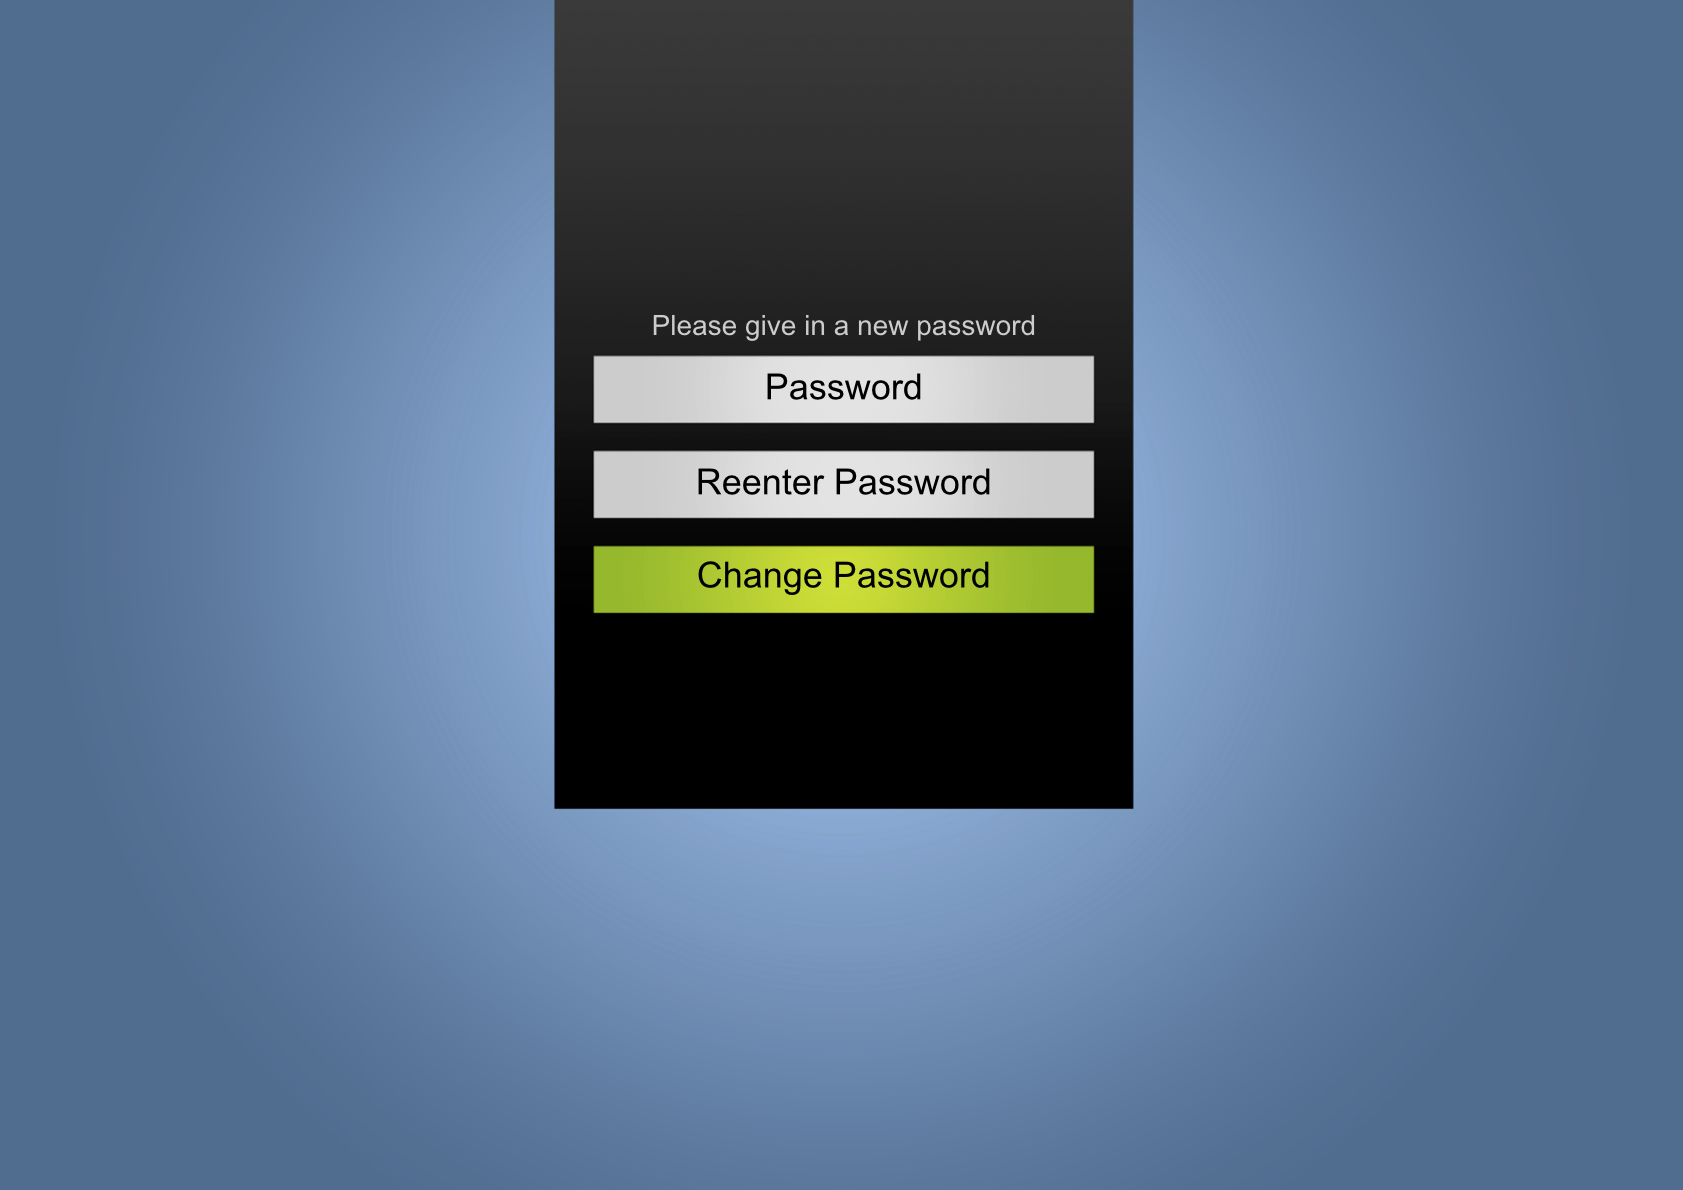
\includegraphics[scale=0.4]{img/Calzonelostpassword2}}
\label{fig:CalZone Lost Password 2}
\end{figure}
\end{center}

%Ingeschreven vakken aanpassen
\subsubsection{Ingeschreven vakken aanpassen}
\noindent\begin{table}[H]
            \begin{tabular}{l | p{10cm}}
                \textbf{ID:} & FR1.4\\ \hline
                \textbf{TITEL:} & Ingeschreven vakken aanpassen\\ \hline
                \textbf{PRIORITEIT:} &  Hoog \\ \hline
                \textbf{PREREQUISITIES:} & \\ \hline
                \textbf{TOEGANG:} &  Aangemelde Student \\ \hline
                \textbf{BESCHRIJVING:} & Een aangemelde student kan de vakken waarvoor deze is ingeschreven tijdelijk aanpassen. 
                						Dit betekent dat de aangemelde student zich kan uitschrijven voor vakken waar hij op ingeschreven is en  zich kan inschrijven voor vakken waarvoor hij nog niet is ingeschreven.\\
            \end{tabular}\\
            \caption{FR1.4 - Ingeschreven vakken aanpassen}
            \label{tab:FR1.4 - Ingeschreven vakken aanpassen}
        \end{table}
        
\textbf{Stappenplan:}
\begin{itemize}
\item Voor het inschrijven:
	\begin{enumerate}
	\item De aangemelde student (voortaan student geheten) ziet zijn persoonlijke hoofdpagina (zie figuur \ref{fig:CalZone Profile}). Bovenaan ziet hij de optie om zich in te schrijven voor vakken.
	\item De student klikt op deze optie en wordt doorverwezen naar een nieuw venster waar zich kan in schrijven voor vakken (zie figuur \ref{fig:CalZone Enroll}).
	\item De student vult een zoekterm in. Deze zoekterm verwijst naar het vak waarvoor hij zich wil inschrijven. 
	\item De student klikt op de knop met de naam "Zoek vak". Er verschijnt in hetzelfde venster een tabel met gevonden vakken die voldoen aan de zoekterm voor de faculteit en richting. In die tabel kan je minstens de naam en de titularis van het vak bezichtigen.
	\item De student selecteert in de tabel het gewenste vak. Hierdoor verschijnt er een melding met de vraag of de student zeker is dat hij voor dit vak wil inschrijven.
	\item De student klikt op "ja" en is nu ingeschreven voor het vak. Vanaf nu verschijnt het vak in zijn persoonlijk lesrooster en in de lijst van ingeschreven vakken.
	\end{enumerate}
	
\item Voor het uitschrijven:
	\begin{enumerate}
	\item De aangemelde student (voortaan student geheten) ziet zijn persoonlijke hoofdpagina (zie figuur \ref{fig:CalZone Profile}) in zijn browser. Bovenaan ziet hij de optie om zich uit te schrijven voor vakken.
	\item De student klikt op deze optie en wordt doorverwezen naar een nieuw venster waar hij een lijst van al zijn vakken ziet (zie figuur \ref{fig:CalZone Enrolled}). Naast elk vak bevindt er zich een knop met de naam "Uitschrijven".
	\item De student klikt op de knop naast het gewenste vak waarvoor hij wilt uitschrijven. Vervolgens verschijnt er een melding op het scherm met de vraag of hij zeker is of hij zich wilt uitschrijven voor dit vak.
	\item De student klikt op \"ja\" en is nu uitgeschreven voor dit vak en wordt teruggestuurd naar zijn persoonlijk lesrooster. Voortaan verschijnt het betreffende vak niet meer in zijn persoonlijk lesrooster noch in zijn lijst van ingeschreven vakken. en dan kan de gebruiker in de lijst van vakken zoeken op naam en vaknummer en wordt dan naar een pagina doorgestuurd waarop deze in lijstvorm te zien zijn.
	\end{enumerate}
\end{itemize}

%TODO
\textbf{Uitzonderingen:}
\begin{itemize}
\item De student wilt inschrijven voor een vak waar hij reeds voor is ingeschreven.
\item De zoekopdracht van de student vindt geen vakken.

\end{itemize}

\begin{center}
\begin{figure}[H]
\caption{CalZone Enroll}
\centerline{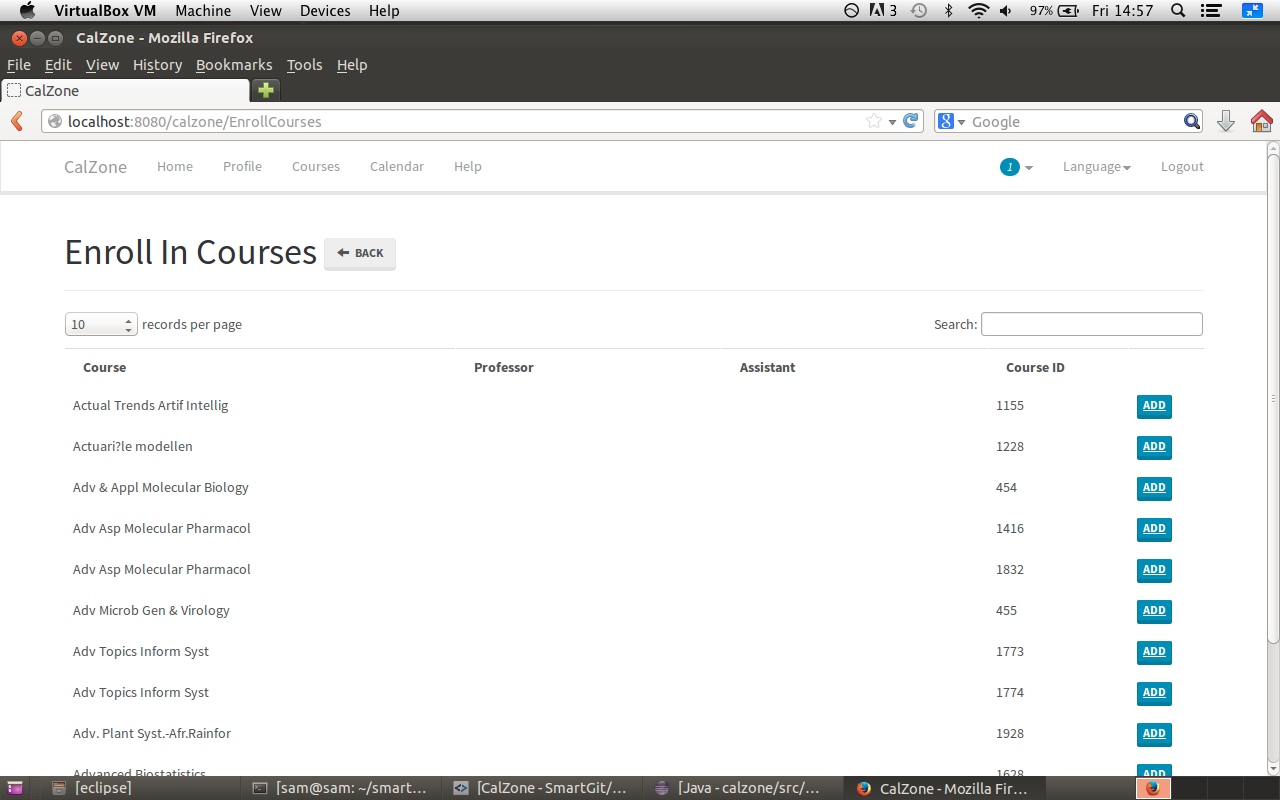
\includegraphics[scale=0.4]{img/CalzoneEnroll}}
\label{fig:CalZone Enroll}
\end{figure}
\end{center}

%Taal aanpassen
\subsubsection{Taal aanpassen}
\noindent\begin{table}[H]
            \begin{tabular}{l | p{10cm}}
                \textbf{ID:} & FR1.5 \\ \hline
                \textbf{TITEL:} & Taal aanpassen\\ \hline
                \textbf{PRIORITEIT:} &  Laag \\ \hline
                \textbf{PREREQUISITIES:} & \\ \hline
                \textbf{TOEGANG:} &  Aangemelde gebruiker \\ \hline
                \textbf{BESCHRIJVING:} & Een aangemelde gebruiker kan zijn taal van voorkeur aanpassen zodat de applicatie wordt weergegeven in een andere taal.\\
            \end{tabular}\\
            \caption{FR1.5 - Taal aanpassen}
            \label{tab:FR1.5 - Taal aanpassen}
        \end{table}
        
\textbf{Stappenplan:}
\begin{itemize}

\item Voor niet aangemelde gebruiker:
	\begin{enumerate}
	\item De niet aangemelde gebruiker (voortaan gebruiker geheten) ziet de CalZone hoofdpagina (zie figuur \ref{fig:CalZone Home}) in zijn webbrowser.Links onder ziet deze de optie om de taal aan te passen.
	\item De gebruiker klikt op deze optie en krijgt een scroll lijst te zien met daarin de mogelijke talen waarin CalZone beschikbaar is. Deze lijst bevat minstens de taal Engels en Nederlands.
	\item De gebruiker klikt op zijn gewenste taal en terug doorverwezen naar de CalZone hoofdpagina (zie figuur \ref{fig:CalZone Profile}) en ziet de applicatie nu in de geselecteerde taal. 
	\end{enumerate}

\item Voor alle andere gebruikers, behalve de programmabeheerder:
	\begin{enumerate}
	\item De aangemelde gebruiker (voortaan gebruiker geheten) ziet zijn persoonlijke hoofdpagina (zie figuur \ref{fig:CalZone Profile}) in zijn webrowser. Bovenaan ziet hij een optie om zijn account gegevens aan te passen.
	\item De gebruiker klikt op deze optie en word doorverwezen naar een webpagina met al zijn persoonlijke informatie. Hierbij staat de optie "taalkeuze". 
	\item De gebruiker klikt op deze optie en er verschijnt een scroll lijst met daarin de mogelijke talen waarin CalZone beschikbaar is. Deze lijst bevat minstens de taal Engels en Nederlands.
	\item De gebruiker klikt op zijn gewenste taal en wordt doorverwezen naar zijn persoonlijke hoofdpagina (zie figuur \ref{fig:CalZone Profile}) en ziet de applicatie nu in de geselecteerde taal. Het systeem onthoudt deze wijziging zolang deze niet opnieuw door de gebruiker zelf wordt aangepast.
	\end{enumerate}
	
\item Voor de programmabeheerder:
	\item De programmabeheerder ziet zijn beginvenster in zijn webbrowser. Rechts ziet hij de optie om de taal van de applicatie te wijzigen.
	\item De programmabeheerder klikt op deze optie en wordt doorverwezen naar een nieuwe pagina. 
	\item De programmabeheerder herhaalt stappen 2 en 3 van de andere gebruikers om zijn taal te wijzigen.
\end{itemize}

%TODO eventuele uitzonderingen

%Afmelden
\subsubsection{Afmelden}
\noindent\begin{table}[H]
            \begin{tabular}{l | p{10cm}}
                \textbf{ID:} & FR1.6 \\ \hline
                \textbf{TITEL:} & Afmelden\\ \hline
                \textbf{PRIORITEIT:} &  Hoog \\ \hline
                \textbf{PREREQUISITIES:} & \\ \hline
                \textbf{TOEGANG:} &  Aangemelde gebruiker \\ \hline
                \textbf{BESCHRIJVING:} & Een aangemelde gebruiker moet zijn sessie kunnen be\"{e}indigen door zich af te melden.\\
            \end{tabular}\\
            \caption{FR1.6 - Afmelden}
            \label{tab:FR1.6 - Afmelden}
        \end{table}
\textbf{Stappenplan:}
\begin{enumerate}
\item De aangemelde gebruiker ziet zijn persoonlijke hoofdpagina (zie figuur \ref{fig:CalZone Profile}) in zijn webbrowser. Rechts boven ziet hij de optie om af te melden.
\item De gebruiker klikt op deze optie en wordt uitgelogd. Hij krijgt de melding dat hij uitgelogd is en krijgt het beginscherm (zie figuur \ref{fig:CalZone Home}) van de niet-aangemelde gebruiker te zien.
\end{enumerate} 

%Profiel gegevens aanpassen
\subsubsection{Profiel gegevens aanpassen}
\noindent\begin{table}[H]
            \begin{tabular}{l | p{10cm}}
                \textbf{ID:} & FR1.7 \\ \hline
                \textbf{TITEL:} & Profielgegevens aanpassen\\ \hline
                \textbf{PRIORITEIT:} &  Medium \\ \hline
                \textbf{PREREQUISITIES:} & \\ \hline
                \textbf{TOEGANG:} & Aangemelde gebruiker \\ \hline
                \textbf{BESCHRIJVING:} & Een gebruiker kan zijn profielgegevens aanpassen. Meer bepaald kan hij de volgende informatie aanpassen:
                                        \begin{itemize}\itemsep1pt \parskip0pt \parsep0pt
                                        \item Naam
                                        \item Voornaam
                                        \item Gebruikersnaam
                                        \item Wachtwoord
                                        \item Geboortedatum
                                        \item Email
                                        \end{itemize}\\
            \end{tabular}\\
            \caption{FR1.7 - Profiel gegevens aanpassen}
            \label{tab:FR1.7 - Profielgegevens aanpassen}
        \end{table} 
               
\textbf{Stappenplan:}
\begin{enumerate}
\item De aangemelde gebruiker ziet zijn beginvenster (zie figuur \ref{fig:CalZone Profile}) in zijn webbrowser. Bovenaan ziet hij de optie om zijn profielgegevens te bezichtigen.
\item De gebruiker klikt deze optie aan en wordt doorverwezen naar een nieuwe pagina. Hierop ziet hij al zijn profielgegevens in tekstvelden. De gebruiker kan de gegevens opgesomd in de beschrijving hierboven wijzigen in de tekstvelden.
\item De gebruiker wijzigt de gewenste velden aan en ziet een knop met de naam "Wijzigingen opslaan" om deze permanent te wijzigen.
\item De gebruiker klikt op deze knop en de gegevens zijn permanent gewijzigd.
\end{enumerate}

%TODO eventuele uitzonderingen

%Beschikbaarheidsformulier aanmaken 
\subsubsection{Beschikbaarheidsformulier aanmaken}  
\noindent\begin{table}[H]
            \begin{tabular}{l | p{10cm}}
                \textbf{ID:} & FR1.8 \\ \hline
                \textbf{TITEL:} & Beschikbaarheidsformulier aanmaken\\ \hline
                \textbf{PRIORITEIT:} &  Laag \\ \hline
                \textbf{PREREQUISITIES:} & \\ \hline
                \textbf{TOEGANG:} & Assistent, Professor \\ \hline
                \textbf{BESCHRIJVING:} & Een gebruiker (van het type beschreven in toegang) heeft de optie om een formulier in te dienen waarin hij aangeeft wat zijn vrije momenten zijn om les te geven. De scheduler houdt hier dan rekening mee bij het opstellen van de lesroosters.\\ 
            \end{tabular}\\
            \caption{FR1.8 - Beschikbaarheidsformulier aanmaken}
            \label{tab:FR1.8 - Beschikbaarheidsformulier aanmaken}
        \end{table}
        
%Meertaligheid voorzien
\subsubsection{Meertaligheid voorzien}  
\noindent\begin{table}[H]
            \begin{tabular}{l | p{10cm}}
                \textbf{ID:} & FR1.9 \\ \hline
                \textbf{TITEL:} & Meertaligheid voorzien\\ \hline
                \textbf{PRIORITEIT:} &  Hoog \\ \hline
                \textbf{PREREQUISITIES:} & \\ \hline
                \textbf{TOEGANG:} & Aangemelde gebruiker \\ \hline
                \textbf{BESCHRIJVING:} & Een gebruiker (van het type beschreven in toegang) moet de optie hebben op zijn taal aan te passen. Het programma zal minstens over 2 talen beschikken, namelijk Engels en Nederlands\\ 
            \end{tabular}\\
            \caption{FR1.9 - Meertaligheid voorzien}
            \label{tab:FR1.9 - Meertaligheid voorzien}
        \end{table}
        
%Automatisch Inloggen
\subsubsection{Automatisch Inloggen}  
\noindent\begin{table}[H]
            \begin{tabular}{l | p{10cm}}
                \textbf{ID:} & FR1.10 \\ \hline
                \textbf{TITEL:} & Automatisch Inloggen\\ \hline
                \textbf{PRIORITEIT:} &  Medium \\ \hline
                \textbf{PREREQUISITIES:} & Gebruiker moet zich al eens ingelogd hebben \\ \hline
                \textbf{TOEGANG:} & Aangemelde gebruiker \\ \hline
                \textbf{BESCHRIJVING:} & Een gebruiker (van het type beschreven in toegang) kan automatisch ingelogd worden als deze terugkomt naar de website van CalZone. 
            \end{tabular}\\
            \caption{FR1.10 - Automatisch Inloggen}
            \label{tab:FR1.10 - Automatisch Inloggen}
        \end{table}
        
%Profiel verwijderen
\subsubsection{Profiel verwijderen}
	\begin{table}[H]
	\caption{FR1.11 - Profiel aanmaken}
    		\begin{tabular}{l | p{10cm}}
        \textbf{ID:} & FR1.11 \\ \hline
        \textbf{TITEL:} & Profiel verwijderen \\ \hline
        \textbf{PRIORITEIT:} &  Laag \\ \hline
        \textbf{PREREQUISITIES:} & Gebruiker moet al een account hebben\\ \hline
        \textbf{TOEGANG:} &  Aangemelde Gebruiker \\ \hline
        \textbf{BESCHRIJVING:} & Een gebruiker kan zijn account verwijderen\\
    \end{tabular} 
	\label{tab:FR1.11 -Profiel aanmaken}
\end{table}

\textbf{Stappenplan:}
\begin{enumerate}
\item Een aangemelde gebruiker kan bij profiel gegevens kiezen voor de optie \"account verwijderen\".
\item De gebruiker klikt hierop en er verschijnt een waarschuwingsbericht waarin staat of hij zeker is dat hij zijn account wil verwijderen.
\item De gebruiker klikt op \"ja\" en word terug naar het beginvenster (zie figuur \ref{fig:CalZone Home}) gebracht.
\end{enumerate}

%Opnieuw Confirmatie Mail Sturen
\subsubsection{Confirmatie Mail Herzenden}
	\begin{table}[H]
	\caption{FR1.12 - Confirmatie Mail Herzenden}
    		\begin{tabular}{l | p{10cm}}
        \textbf{ID:} & FR1.12 \\ \hline
        \textbf{TITEL:} & Confirmatie Mail Herzenden \\ \hline
        \textbf{PRIORITEIT:} &  Laag \\ \hline
        \textbf{PREREQUISITIES:} & Gebruiker moet al een account hebben\\ \hline
        \textbf{TOEGANG:} &  Niet-aangemelde Gebruiker \\ \hline
        \textbf{BESCHRIJVING:} & Een gebruiker heeft de mogelijkheid opnieuw zijn emailadres op te geven, om opnieuw een confirmatie mail te versturen. Nodig wanneer activatie-mail na registratie verloren is gegaan\\
    \end{tabular} 
	\label{tab:FR1.12 -Profiel aanmaken}
\end{table}

\textbf{Stappenplan:}
\begin{enumerate}
\item Gebruiker bevind zich op de registratie pagina, hierop bevind zich een link naar de pagina om een activatie mail te herzenden.
\item Gebruiker klikt op link.
\item De gebruiker komt op een pagina terecht om zijn emailadres in te vullen en zo de registratie-mail nog eens te verzenden.
\end{enumerate}

%Volgende Les Snel Bekijken
\subsubsection{Volgende Les Op Profiel Pagina}
	\begin{table}[H]
	\caption{FR1.13 - Volgende Les Op Profiel Pagina}
    		\begin{tabular}{l | p{10cm}}
        \textbf{ID:} & FR1.13 \\ \hline
        \textbf{TITEL:} & Volgende Les Op Profiel Pagina \\ \hline
        \textbf{PRIORITEIT:} &  Medium \\ \hline
        \textbf{PREREQUISITIES:} & Gebruiker moet al een account hebben\\ \hline
        \textbf{TOEGANG:} &  Aangemelde Gebruiker \\ \hline
        \textbf{BESCHRIJVING:} & Een aangemelde gebruiker kan op zijn profiel pagina meteen zien wat zijn volgende les is, waar deze plaats vind en om hoe laat deze begint. Deze word steeds ge-update zodat de eerst volgende les getoond wordt. \\
    \end{tabular} 
	\label{tab:FR1.13 -Profiel aanmaken}
\end{table}
\clearpage
